\section{Droplet formation}

Microfluidics is the control and study of fluids in the micrometre scale, in which one subdivision of microfluidics is droplet-based microfluidics \parencite{Atencia2004, Stone2004}. Droplet-based systems use immiscible phases to create discrete volumes of droplets. The two-phase flow microfluidics, where the droplets flow in closed microchannels \parencite{Pit2015}. Microfluidic systems are characterised or described by the low Reynolds number flow regime which requires that all fluid flow is essentially laminar. The devices are usually fabricated in glass, plastic or various polymers and extend in only a few square centimetres in size. \parencite{Zhu2017,Pit2015,Cole2015} \\

\noindent Micro- or nanometre-sized droplets have come into the spotlight due to their great potential to provide new breakthroughs for scientists in the field of nanoparticle synthesis and diagnostic testing. \parencite{Jeevanandam2018,Bayda2019} To make droplets, top-down emulsification techniques have been conventionally used. The variation in droplet size, however, is relatively big for the conventional methods, and a droplet separation process is required to collect mono-dispersed droplets. Recently, microfluidics has been recognised as a promising alternative to the conventional methods. \parencite{SHARMA2021} To achieve more ductile droplet generation, external electrical or mechanical forces can be applied. Here, droplet-based microfluidics involves the generation and manipulation of discrete droplets inside micro-devices. \parencite{Jensen2004,Belder2005} Hence, as opposed to the conventional methods, this method produces highly mono-disperse droplets in the nanometre to micrometre diameter range, at rates of up to 20.000/second. \parencite{Kobayashi2007} 


\noindent When generating droplets, it is essential to produce droplets of controlled size. Droplet size is an highly important parameter as it controls the efficiency of encapsulation of individual cells and biomolecules and rates of reaction \parencite{Shepherd2021}. From a fundamental point of view, droplet size dictates the mixing dynamics \parencite{Song2006,Huebner2011,Wang2016} flow resistance \parencite{Bithi2010,Baroud2010}, breakup \parencite{Leshansky2012,Hoang2013}, coalescence (the process by which two or more droplets or particles merge during contact to form a single daughter droplet) \parencite{Bithi2014}, and collective behaviour \parencite{Janssen2012,Bithi2015}. Since experimental conditions including flow rates, fluid properties and channel dimensions may vary for different applications, it is important to understand drop formation and develop predictive models of how system parameters influence droplet size.


In general, the strength of droplet-based applications lies in mono-dispersity of the size of the droplets to ensure reliability and reproducibility \parencite{Zhu2017}. 

Basically, in droplet formations, there exist two immiscible phases, referred to as the continuous phase and dispersed phase. The flow rate ratio of the continuous phase and dispersed phase, interfacial tension between two phases, and the geometry of the channels used for droplet generation can affect the size of the micro droplets. \parencite{Gu2011,Sharma2012}

Generally, the micro-droplet generation methods can be classified into passive and active. In active methods an external energy such as electric, magnetic, or centrifugal is needed. Passive droplet formation methods are simple and common. The geometries of passive micro-droplet generation include cross-flowing, flow focusing and co-flowing.  Working with low Reynold's numbers ensures a laminar flow in the droplet-based microfluidic devices. \parencite{Zhu2017,Zhu2019} The Reynolds number for flow in a pipe or tube is given by 

\begin{equation*}
Re = \frac{\rho V D}{\mu}    
\end{equation*}

\noindent Where $\rho$ is the density of the fluid ($kg/m^3$), V is the flow speed (m/s), D is the pipe diameter (m), and $\mu$ is the dynamic viscosity of the fluid ($Pa \cdot s$). \parencite{rothmayerfundamentals} 

\noindent Droplet microfluidics provides a unique method for fabrication of mono-disperse microparticles with control over the size, morphology, and functionality, in a high throughput manner. \parencite{Zhu2017, Zhu2019}

Mono-disperse emulsion droplets produced via droplet microfluidics in their natural state maintain a spherical shape due to the minimization of their surface energy. In the simplest case, polymeric micro-spheres or microgels composed of either polymer chains or cross-linked polymer networks can be obtained by solidification of single emulsion droplets. \parencite{Choi2019,2020} Production of mono-disperse micro-particles with well-defined sizes, mechanical properties, and functionalities have an enormous impact on biomedical applications such as drug delivery and cell encapsulation. For instance, polymeric microspheres or microgels prepared via droplet microfluidics enable flexible delivery of drugs as particle size and material composition strongly affects their release profile, biodistribution, and administration route. Moreover, encapsulation of cells in microgels provide a biocompatible 3D micro-environment for living cells by protecting the cells from the surroundings while simultaneously supplying adequate amount of water, oxygen, and nutrients required to sustain the cells. \parencite{Zhu2017,Kim2013,Zhu2019,Utech2015} 


\subsection{Forces Acting on Fluid Flow}
Microfluidic devices offer an alternate and versatile route to produce emulsions. An emulsion is produced in a microfluidic device by precisely fabricating one drop at a time. This process is an outcome of a well-controlled balance between various forces acting on the fluid flow. These forces include inertial force, viscous force, interfacial tension, and buoyancy. In some cases, external forces such as electric magnetic and centrifugal forces are also utilised. The balance of these forces determines the fluid behaviour and thus the mechanism of droplet formation. Typically, in microfluidic systems, buoyancy is small compared to interfacial and viscous forces during droplet formation due to the relatively small channel size, flow velocity and droplet volume. Therefore, the complex phenomenon of droplet breakup is determined by various dimensionless numbers, which are related to the fluid properties, channel geometries, and the flow conditions. \parencite{Zhang2016,Zhu2019,Zhu2017}

Capillary number (Ca) and Weber number (We) are two main dimensionless numbers that determine the flow behaviour in the channel. The capillary number represents the relative effect of viscous forces and surface tension, while the Weber number reflects the balance between inertial and surface tension forces. For instance, in a single emulsion system comprising of a dispersed phase and a continuous phase, Ca of the continuous phase and We of the dispersed phase are typically low, yielding formation of droplets one by one, which is the dripping mode. \parencite{Zhang2016,Zhu2019,Zhu2017}
\blankline

\noindent In order to create droplets, several droplet generation mechanisms have been introduced. As already mentioned, the most commonly used devices are cross-flow, flow-focusing, and co-flow. \parencite{Zhu2017,Pit2015}

In flow-focusing and co-flow microfluidic devices, droplet generation is the result of the shear stress of a continuous phase on a dispersed phase, while in T-junction devices, droplet generation is caused by the pressure of a continuous phase on a dispersed phase. \parencite{Zhu2019,Zhu2017}

Both phases are usually immiscible liquids. The dispersed phase is hydrophilic, biocompatible, and can be a stream of cells suspended in a polymer. The continuous phase can be a nontoxic oil or an aqueous solution of lower viscosity than the dispersed phase. As the continuous phase meets the dispersed phase, shear stress and pressure cause the dispersed phase to pinch-off and form droplets. The continuous phase serves as the carrier for the dispersed phase, and it should contain a surfactant to lower the surface tension of hydrogels, reduce the wettability at channel walls, and act as a stabilizer for the produced emulsion.
To obtain stable operation, it is important to match the material properties with the fluids being used.\parencite{Zhu2019,Zhu2017}

\subsection{Tuning Parameters}
In this subsection, the three parameters that are used to tune in order to achieve the desired properties for droplet formation. 

\subsubsection{Wettability}
Two possible conditions can occur when two immiscible fluids come in contact with a substrate: either one liquid preferentially wets the wall and separates the other from the surface, or both liquids are partially wetting and an equilibrium angle is found. Due to the close proximity of the walls to the two phases, the wetting conditions strongly influence the formation and transport of droplets in microchannels. It is essential that the continuous phase preferentially wets the walls to produce stable flow regimes. If this is not the case, then droplets can get stuck as the two phases flip between wetting the walls and device operation is completely irreproducible. The thin film that forms under preferentially wetting separates the droplets from the microchannel wall which helps lubricate their motion and compartmentalize the contents. \parencite{Christopher2007}

One of the most common materials used for microfluidic chip fabrication is Polydimethylsiloxane (PDMS) and it is naturally hydrophobic, so the oil phase wets the walls in water/oil emulsions. However, PDMS can be turned hydrophilic through plasma treatment when bonding it to another substrate during the soft lithography fabrication process. \parencite{Zhu2017,Christopher2007}

\subsubsection{Interfacial Tension} 
Surface tension arises because of an imbalance of forces on the fluid molecules near the interface when two immiscible phases come in contact. Molecules in the interior are completely surrounded by molecules of the same type so external forces balance. At the interface the molecules are exposed to both phases, and the attractive force of its own molecules creates a net force that draws the molecules inward. \parencite{Peng2011,Lee2021,Shui2009}

This force is in turn balanced by the fluid’s resistance to compression. As a consequence of the force balance, the interface attempts to minimize its surface energy by reducing the interfacial area and ends up taking on a spherical shape. \parencite{Peng2011,Lee2021,Shui2009}

\subsubsection{Surfactants}
Surfactants have both hydrophobic and hydrophilic parts which makes them soluble in both organic and aqueous phases causing them to migrate and become trapped at an interface. The main purpose of adding surfactants is to lower the surface tension at the interface and to stabilize droplets against coalescence. Hence, selecting the appropriate surfactant is important for making stable droplets. \parencite{Baret2012,Kovalchuk2018}

\subsection{Types of Microfluidic Geometries}
In this subsection, the three most commonly used geometries for droplet generation will be explained in short. 


\subsubsection{Cross-flow}  
T-junction devices belong to the cross-flow geometry in microfluidics and is one of the most common microfluidic geometry employed to generate droplets. The geometry is easy to fabricate, operate and to create consistent droplets of relatively high mono-dispersity. \parencite{Zhu2017} The easily controllable production of a single stream of mono-disperse droplets in a microfluidic channel was first demonstrated using a T-channel geometry, initially proposed by Thorsen et al in 2001. \parencite{Thorsen2001}

\begin{figure}
 \centering
 \begin{subfigure}[b]{0.45\textwidth}
   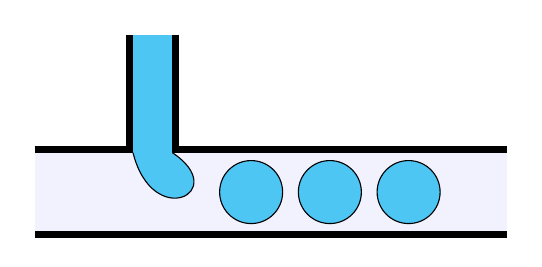
\begin{tikzpicture}


%definitions

\def\x{3} %pipe length
\def\y{0.5} % pipe half-width
\def\r{0.4} % drop radius
\def\w{5} %width line

%
%FIG1
%

%main pipe

\draw[line width=\w] (-\x,\y) -- (-\x/2-\y/2,\y) -- (-\x/2-\y/2,\y+\x/2); %upper pipe + left co-pipe
\draw[line width=\w] (-\x/2+\y/2,\y+\x/2) -- (-\x/2+\y/2,\y) -- (\x,\y); %right co-pipe + upper pipe
\draw[line width=\w] (-\x,-\y) -- (\x,-\y); %lower pipe contour

\fill[fill=blue!5] (-\x,-\y) rectangle (\x,\y); %main pipe fill

\fill[fill=cyan!70](-\x/2-\y/2-0.001,\y-0.001) rectangle (-\x/2+\y/2,\y+\x/2); % co-pipe fill

\filldraw[thin,fill=cyan!70] (-\x/2-\y/2,\y) .. controls (-\x/2,-\y) and (-\x/2+2*\y,0) ..  (-\x/2+\y/2,\y); % first droplet

\foreach \c in {(0,0), (1,0), (2,0)} \filldraw[thin,fill=cyan!70] (-\x/2+2.5*\y,0) + \c circle (\r); %drops


\end{tikzpicture}
   \caption{} \label{fig:a}
 \end{subfigure}
    \hfill
    \begin{subfigure}[b]{0.45\textwidth}
    \begin{tikzpicture}


%definitions

    \def\x{2.7} %pipe length
    \def\y{0.5} % pipe half-width
    \def\r{0.4} % drop radius

    \def\s{\x/4} %shift
    \def\o{0.2} %smooth offset

    \def\w{5}

%
%FIG2
%

    \draw[line width = \w, name path=L] (-\x/2-\y/2-\s,\y+\x/2) -- (-\x/2-\y/2,\y) -- (-\x,\y); %left co-pipe + upper pipe
    \draw[line width = \w, name path=R] (-\x/2+\y/2-\s,\y+\x/2) -- (-\x/2+\y/2,\y) -- (\x,\y); %right co-pipe contour + upper pipe
    \draw[line width = \w] (-\x,-\y) -- (\x,-\y); %lower pipe contour

    \tikzfillbetween[of=L and R]{cyan!70}; %fill co-pipe
    \draw[line width = \w, white] (-\x/2-\y/2-\s-\o,\y+\x/2) -- (-\x/2+\y/2-\s+\o,\y+\x/2); %smooth

    \fill[fill=blue!5](-\x,-\y) rectangle (\x,\y); %main pipe fill

    \filldraw[thin,fill=cyan!70] (-\x/2-\y/2,\y) .. controls (-\x/2,-\y) and (-\x/2+2*\y,0) ..  (-\x/2+\y/2,\y); % first droplet

    \foreach \c in {(0,0), (1,0), (2,0)} \filldraw[thin,fill=cyan!70] (-\x/2+2.5*\y,0) + \c circle (\r); %drops

%arrows

    \draw[blue, line width = 0.8*\w,-{Triangle[length=6, width=6]}] (-0.9*\x,0) -- (-2*\x/3,0);
    \draw[purple, line width = 0.8*\w,-{Triangle[length=6, width=6]}] (-\x/2-0.5*\s,\y+0.5*\x/2) -- (-\x/2,\y);
    \end{tikzpicture}
    \caption{} \label{fig:b}
    \end{subfigure}
    \hfill
\begin{subfigure}[b]{0.45\textwidth}
    \begin{tikzpicture}


%definitions

    \def\x{2.7} %pipe length
    \def\y{0.5} % pipe half-width
    \def\r{0.4} % drop radius

    \def\s{\x/2} %shift
    \def\w{5} %width
    \def\o{0.2} %offset

%
%FIG3
%

    \coordinate (A) at (\x,\y);
    \coordinate (B) at (-\x/2+\y/2,\y);
    \coordinate (C) at (-\x/2 + \y/2 -\s,\y+\s);
    \coordinate (D) at (-\x/2 - \y/2 -\s,\y+\s);
    \coordinate (E) at (-\x/2+\y/2,0);
    \coordinate (F) at (-\x/2-\y/2-\s,-\y-\s);
    \coordinate (G) at (-\x/2+\y/2-\s,-\y-\s);
    \coordinate (H) at (-\x/2+\y/2,-\y);
    \coordinate (I) at (\x,-\y);


%main pipe

%straight section

    \draw[line width = \w, name path=U1] (B) -- (A); %upper pipe
    \draw[line width = \w, name path = D1] (H) -- (I); %lower pipe contour



%tilted section

    \draw[line width = \w, name path=U] (F) -- (E); %upper pipe contour 
    \draw[line width = \w, name path=D] (G) -- (H); %lower pipe contour

    \tikzfillbetween[of=U and D]{blue!5}; %tilted main pipe fill
    \draw[line width = \w, white] (-\x/2-\y/2-\s-\o,-\y-\s) -- (-\x/2+\y/2-\s+\o,-\y-\s); %main pipe smooth

%co-pipe

    \draw[line width = \w, name path=L] (D) -- (E); %left co-pipe
    \draw[line width = \w, name path=R] (C) --(B); %right co-pipe

    \tikzfillbetween[of=L and R]{cyan!70}; %co-pipe fill
    \draw[line width = \w, white] (-\x/2 + \y/2 -\s+\o,\y+\s) -- (-\x/2 - \y/2 -\s -\o,\y+\s); %co-pipe smooth
        
    \tikzfillbetween[of=U1 and D1]{blue!5}; %main pipe fill

    \filldraw[thin,fill=cyan!70] (E) .. controls (-\x/2,-\y/2) and (-\x/2+2.5*\y,0) ..  (B); % first droplet

    \foreach \c in {(0,0), (1,0), (2,0)} \filldraw[thin,fill=cyan!70] (-\x/2+2.5*\y,0) + \c circle (\r); %drops

%arrows

    \draw[purple, line width = 0.8*\w,-{Triangle[length=6, width=6]}] (-\x/2 -\s/1.5,\y+\s/1.5) -- (-\x/2 -\s/3,\y+\s/3);
    \draw[blue, line width = 0.8*\w,-{Triangle[length=6, width=6]}] (-\x/2 -\s/1.5,-\y-\s/1.5) -- (-\x/2 -\s/3,-\y-\s/3);
    
\end{tikzpicture}
\caption{} \label{fig:c}
\end{subfigure}%
\caption{M1} \label{fig:M1}

\end{figure}




% \begin{figure} [H]
%     \centering
%     \includegraphics[width=15cm, height=4cm]{Latex/Figurer/DF_Fig_1_tjunction.png}
%     \caption{The figures depicts the various geometry of T and Y-junctions. (a) and (b) are the T-junctions, while (c) is the Y-junction.NEW IMAGE!!!}
%     \label{fig:tjunction}
% \end{figure}

\noindent For water-in-oil droplets; the oil sample (continuous phase) flows in one direction. The aqueous sample (dispersed phase) flows into the oil sample at the T- or Y-junction. An example of T- and Y-junction can be seen in \autoref{fig:M1}. As the aqueous sample joins the oil sample, the shear forces of the oil continuously flowing breaks the aqueous sample into a droplet. Basically, the dispersed phase enters the continuous, shear forces elongate the head of the dispersed phase until a segment eventually separates and relaxes into a sphere due to interfacial tension. In this case, the size of the droplet is determined by parameters such as flow rates and viscosities, channel wall wettability, surfactant and their concentrations, channel dimensions and interfacial tension of the oil sample. The flow rate of the continuous phase (oil in this example) is usually higher than the dispersed phase (water). To achieve oil-in-water droplets, the liquids are reversed. \parencite{Zhu2017}



\subsubsection{Flow-focusing} 
For water-in-oil droplets; the water sample (dispersed phase) meets the oil sample (continuous phase) at the junction, where there is usually a narrowing of the channels at the junction point. Similar to cross-flow, the flow rate of the continuous phase (oil in this example) is usually higher than the flow rate of the dispersed phase (water). In this case, it is possible to increase the size of the droplets by decreasing the flow rate of the continuous phase. To achieve oil-in-water droplets, the liquids are reversed. \parencite{Zhu2017}

% \begin{figure}[H]
%     \centering
%     \includegraphics[width=8cm, height=6cm]{Latex/Figurer/DF_Fig_2_flow focussing.png}
%     \caption{An illustration of the geometry of the flow-focusing device.NEW IMAGE!!!}
%     \label{fig:FlowFocussing}
% \end{figure}

\begin{figure}[h!]
\centering
\begin{tikzpicture}
%definitions

\def\x{3.2} %pipe length
\def\y{0.5} % pipe half-width
\def\r{0.4} % drop radius

\def\w{5} %width

%
%FIG2
%

\coordinate (A) at (\x,\y);
\coordinate (A1) at (0.1*\x,\y);
\coordinate (A2) at (0.1*\x,\y/2);
\coordinate (A3) at (0,\y/2);
\coordinate (A4) at (0,3*\y);
\coordinate (B) at (-\x,\y);
\coordinate (B1) at (-0.4*\x,\y);
\coordinate (B2) at (-0.4*\x,3*\y);
\coordinate (C) at (-\x,-\y);
\coordinate (C1) at (-0.4*\x,-\y);
\coordinate (C2) at (-0.4*\x,-3*\y);
\coordinate (D1) at (0.1*\x,-\y);
\coordinate (D2) at (0.1*\x,-\y/2);
\coordinate (D3) at (0,-\y/2);
\coordinate (D4) at (0,-3*\y);
\coordinate (D) at (\x,-\y);

%Exterior pipe

\draw[line width = \w/2, name path=U] (A) -- (A1) -- (A2) -- (A3) ; %upper pipe
\draw[line width = \w/2, name path=D] (D) -- (D1) -- (D2) -- (D3) ; %lower pipe

\draw[line width = \w/2] (A3) -- (A4);
\draw[line width = \w/2] (D3) -- (D4);


\tikzfillbetween[of=U and D]{blue!5}; %exterior pipe fill

\fill[blue!5] (C2) rectangle (A4);

%First droplet

\filldraw [thin, fill=cyan!70] plot [smooth cycle] coordinates {(-0.4*\x-0.01,\y) (-\x/6,\r/4)  (\x/8,\r/2) (\x/4,+\r) (\x/4+0.7*\r,0.7*\r) (\x/4+\r,0) (\x/4+0.7*\r,-0.7*\r) (\x/4,-\r) (\x/8,-\r/2)  (-\x/6,-\r/4) (-0.4*\x-0.01,-\y)};

%Interior pipe

\draw[line width = \w/2, name path=U1] (B) -- (B1);
\draw[line width = \w/2, name path=D1] (C) -- (C1);

\tikzfillbetween[of=U1 and D1]{cyan!70}; %exterior pipe fill

\draw[line width = \w/4] (B2) -- (B1);
\draw[line width = \w/4] (C2) -- (C1);

%Drops

\foreach \c in {(0.9,0), (1.9,0)} \filldraw[thin,fill=cyan!70] (0.9,0) + \c circle (\r);

%Arrows

\draw[blue, line width = 0.8*\w,-{Triangle[length=6, width=6]}] (-0.2*\x,2.5*\y) -- (-0.2*\x,\y);
\draw[purple, line width = 0.8*\w,-{Triangle[length=6, width=6]}] (-0.9*\x,0) -- (-2*\x/3,0);
\draw[blue, line width = 0.8*\w,-{Triangle[length=6, width=6]}] (-0.2*\x,-2.5*\y) -- (-0.2*\x,-\y);

\end{tikzpicture}
\caption{M2} \label{fig:M2}
\end{figure}

\noindent In a flow-focusing device, a laminar flow dispersed phase moves through a nozzle, or orifice, to flow within a continuous phase as seen in \autoref{fig:M2}. Shear stress is caused by a reduction in the size of the dispersed phase channel at the orifice, at which hydrodynamic flow-focusing occurs. It is important to use a surfactant in the continuous phase to decrease surface tension and prevent coalescence. \parencite{Zhu2017}
\blankline

\noindent One use of a flow-focusing device is the creation of Janus droplets. These droplets are heterogeneous and composed of two miscible solutions with matching viscosities. \parencite{Xu2020} As mentioned before, the fabrication material of flow-focusing devices is highly dependent on cell compatibility. They can be fabricated in PDMS poured onto an SU-8 micropatterned silicon wafer, also known as soft-lithography. PDMS structures are commonly used for cell culture as they allow for the diffusion of oxygen, nutrients, and wastes. Other fabrication methods use glass capillaries from chromatography components that are commercially available, easy to assemble, and easy to clean. Recently, 3D printing technology has been used for the development of microfluidic devices. \parencite{Zhu2017}

It has been shown that increasing the flow rate ratio of the continuous phase to the dispersed phase causes a decrease in droplet size. If a threshold of flow rates is reached, however, a jet of the dispersed phase will form instead of droplets, which decreases the efficiency of micro-encapsulation. Also, increasing the viscosity of the dispersed phase leads to the generation of larger droplets and a narrow size distribution due to a longer pinch-off time. Moreover, better control of droplet size is directly related to orifice diameter. \parencite{Zhu2019}
\blankline

\noindent Another advantage of flow-focusing devices is the feasibility of high-throughput droplet production. Droplet generation frequency can reach several thousand hertz. In general, the production of small-sized droplets at high frequencies is achieved by proper adjustment of flow rates and selection of the orifice diameter. \parencite{Zhu2017,Pit2015}

\subsubsection{Co-flow}
The third commonly used microfluidic device employs the concept of co-flow. An illustration of a Co-flow device can be seen in \autoref{fig:M3}. The underlying ideas and geometries of co-flow and flow-focusing methods are quite similar. In a ‘co-flow’ geometry the dispersed phase channel is enclosed inside a continuous phase channel.  As the dispersed fluid enters the continuous phase fluid, it experiences the shear forces of the continuous phase fluid until it eventually breaks and forms a droplet by dripping or jetting (Rayleigh–Plateau instability). \parencite{Zhu2017, Pit2015}

% \begin{figure}[H]
%     \centering
%     \includegraphics[width=8cm, height=6cm]{Latex/Figurer/DF_Fig_3_co flow.png}
%     \caption{The figure illustrates the geometry of co-flow device.NEW IMAGE!!!}
%     \label{fig:co_flow}
% \end{figure}


\begin{figure}[h!]
\centering
\begin{tikzpicture}
%definitions

\def\x{3.7} %pipe length
\def\y{1.2} % pipe half-width
\def\r{0.4} % drop radius

\def\w{5} %width

%
%FIG2
%

\coordinate (A) at (\x,\y);
\coordinate (B) at (-\x,\y);
\coordinate (C) at (-\x,-\y);
\coordinate (D) at (\x,-\y);
\coordinate (E) at (-\x/3,\y/3);
\coordinate (F) at (-\x,\y/3);
\coordinate (G) at (-\x,-\y/3);
\coordinate (H) at (-\x/3,-\y/3);

%Exterior pipe

\draw[line width = \w, name path=U1] (B) -- (A); %upper pipe
\draw[line width = \w, name path = D1] (C) -- (D); %lower pipe

\tikzfillbetween[of=U1 and D1]{blue!5}; %exterior pipe fill

%First droplet

\filldraw [thin, fill=cyan!70] plot [smooth cycle] coordinates {(-\x/3-0.05,\y/3) (-\x/6,\r/4) (0,+\r) (0.7*\r,0.7*\r) (+\r,0) (0.7*\r,-0.7*\r) (0,-\r)  (-\x/6,-\r/4) (-\x/3-0.05,-\y/3)};

%Interior pipe

\draw[line width = \w, name path=U] (E) -- (F); %upper pipe
\draw[line width = \w, name path = D] (G) -- (H); %lower pipe

\tikzfillbetween[of=U and D]{cyan!70}; %interior pipe 


%Drops

\foreach \c in {(0,0), (1,0), (2,0)} \filldraw[thin,fill=cyan!70] (-\x/2+2.5*\y,0) + \c circle (\r);

%Arrows

\draw[purple, line width = 0.8*\w,-{Triangle[length=6, width=6]}] (-0.9*\x,2*\y/3) -- (-2*\x/3,2*\y/3);
\draw[blue, line width = 0.8*\w,-{Triangle[length=6, width=6]}] (-0.9*\x,0) -- (-2*\x/3,0);
\draw[purple, line width = 0.8*\w,-{Triangle[length=6, width=6]}] (-0.9*\x,-2*\y/3) -- (-2*\x/3,-2*\y/3);

\end{tikzpicture}
\caption{M3} \label{fig:M3}
\end{figure}


\noindent If droplet break-up happens near the tip of the nozzle, the breakup is called dripping; dripping generates droplets that are highly mono-disperse.  On the other hand, if droplet break-up happens from an extended thread downstream of the nozzle, the breakup is called; jetting can be highly unstable and irregular at high Reynold numbers. Droplet sizes formed through jetting are related to the channel dimensions and the ratio of flow rates. \parencite{Zhu2017, Pit2015}

Although surfactants are commonly used to create stable emulsions, the use of a surfactant could be eliminated in a co-flow device. The laminar flow of the two phases in a co-flow device can be used to generate droplets with amphiphilic properties. In addition, co-flow devices can be used to generate double emulsion droplets or multicomponent droplets that could be used for co-encapsulation and micro-reactions with precise control of the number of inner droplets. \parencite{Zhu2017,Cole2015}

Typically, co-flow devices are fabricated from commercial glass capillaries in which a circular capillary is placed concentrically in a square or circular outer flow tube and less frequently from PDMS. Devices made from glass capillaries exhibit excellent chemical resistance when organic solvents are used, such as tetrahydrofuran and chloroform, which greatly swell PDMS as mentioned before in regard with the other geometries. \parencite{Zhu2017, Pit2015,Cole2015} 

\subsection{Physics behind}
% We will adr

The driven physics behind flow of fluids in microfluidic systems are the Navier-Stokes equations.It is, however, of importance to introduce some concepts/parameters/variables before the Navier-Stokes equations are presented, since the equations are defined/applied accordingly.....

%We focus on cases where continuous phase fluids preferentially wet the channel walls, so that the dispersed droplets are completely surrounded by continuous fluids and outline the governing equations and fundamental dimensionless parameters for droplet generation in two-phase flow system.

%DIMENSIONLESS NUMBERS
%Fluid motions with various characteristics could occur in microflows, which are normally determined by competing physical effects, such as force balance. Dimensionless numbers characterise the relative predominance of different effects and are capable of contrasting flows in parameter space, thereby unifying flowing features between different systems. 
%In order to examine the key dimensionless numbers characterising the droplet, we need to begin with the governing equations that determine microfluidic two-phase flows.

%Liquid-liquid two-phase microflows are well described with the continuum hypothesis. The incompressible continuity equation reads, for both dispersed and continuous phase fluids:
\begin{equation}\label{eq:conti}
    \nabla \cdot \bold{u_{s}} = 0
\end{equation}
%where $\nabla$ is the del operator, $\bold{u_s}$ is the velocity vector of the fluid, and the subscript "s" denoted either "d" or "c", corresponding to dispersed or continuous phase fluid, respectively.
%The momentum equation is the well-known Navier-Stokes equation of incompressible Newtonian fluids:
\begin{equation}\label{eq:ns_incom newton}
    \rho_s \frac{\partial \bold{u_s}}{\partial t} + \rho_s \bold{u_s} \cdot \nabla \bold{u_s} = -\nabla p_s + \eta_s \nabla^2 \bold{u_s} + \bold{f_s}
\end{equation}
%where \textit{t} is the time, $\rho$ the density of the fluid, \textit{p} the pressure, $\eta$ the dynamic shear viscosity, and $\mathbf{f}$ the body force vector per unit volume. Here, the left side of \ref{eq:ns_incom newton} describes inertial acceleration composed of time-dependent acceleration $\rho_s \bold{\partial u_s}/ \partial t$ and convective acceleration $\rho_s \bold{u_s \cdot \nabla u_s}$ (spatial effect), while the right side represents force densities (force per unit volume) (REF:28??pasact).
%The diffusion term $\eta_s \bold{\nabla^2 u_s}$ is the divergence of viscous stresses $\bold{\sigma_s}=\eta_s \left[\bold{\nabla u_s} + \left( \bold{\nabla u_s} \right)^T \right] $. The body force densities $\bold{f_s}$ can cover effects from those like gravity, electrical, magnetic, and centrifugal effects. If no other external fields are applied except gravity, $\bold{f_s}=\rho_s \bold{g}$ with $\mathbf{g}$ being the gravitational acceleration.
%Droplet formation in microfluidic devices involves the deformation and breaking of the liquid-liquid interface. 







%Which type fluid are we talking about: Newtonian or non-Newtonian. Newtonian fluids have a constant viscosity that doesn't change, no matter the pressure being applied to the fluid, This also means they don't compress. As for the non-Newtonian fluids, they are just the opposite- if enough force is applied to these fluids, their viscosity will change. These fluids are broken up into 2 catagories-dilatants, which get thinker when force is applied, and pseudoplastics, which get thinner under the same circumstances.
%These can be further broken into rheopectic and thixotropic categories. Rheopectics work like dilatants in that they get thicker when force is applied. Thixotropic materials get thinner, liek pseudoplastics do.
%The viscosity doesn't change immediately but changes slowly over time as more and more force is applied.
%Water, mineral oil, and alcohol are some example of Newtonian fluid as their viscosity doesn't change with pressure and cannot be compressed. As for the non-Newtonian fluids are divided in further four catagories: dilatants-they become thick or almost solid when force is applied to them and are made up of water mixed with other materials. Oobleck, that are made of cornstarch and water is an example of this dilatants and quicksand is another exampple. The 2nd catagory is the pseudoplastics, where the viscosity changes as new ingredient is added to the mix.Ketchup is one example of such non-Newtonian fluid. 3rd catagory is the rheopectic fluids, that get s thicker in relation to the pressure being applied to them and the time that the pressure is being applied. Example of this type of fluid is cream (with enough time and pressure, cream becomes butter). Thixotorpic is the 4th catagory and is similar to pseudoplastics in that they get thinner as pressure is applied to them, BUT is also dependent on the time that the pressure is being applied. Examples are cosmetic products, asphalt, and glue. 


% \begin{equation}  \label{eq:1}
%     \frac{\partial \rho}{\partial t} + \nabla \cdot (\rho \bold{u}) = 0
% \end{equation}
% \begin{equation}  \label{eq:2}
%     \frac{\partial(\rho \bold{u})}{\partial t} + \nabla \cdot (\rho \bold{uu}) = - \nabla p + \nabla \cdot (\mu \nabla bold{u}) + \bold{F_{\bold{g}+}} \bold{F_{\bold{st}}}
% \end{equation}

%where, $\rho$ is the density, $\bold{u}=(u,v)$ is the velocity vector, $p$ is the pressure, $\mu_{0}$ is the viscosity, and $\phi$ is the surface tension force. To capture the interface between the droplet and the surrounding air, an additional transport equation for the liquid volume fraction is solve. The liquid volume of fraction is denoted by $phi$ and is defined by.

% \begin{equation}
%   \varphi =\begin{cases}
%     1 & \textit{inside the droplet } \\
%     0 & \textit{outside the droplet } \\
%     0 < \varphi < 1 & \textit{at interface cells}
%   \end{cases}
% \end{equation}

%and the transport equation for $\varphi$ is,
% \begin{equation} \label{eq:3}
%     \frac{\partial \phi}{\partial t} + \bold{u} \cdot \nabla \phi = 0
% \end{equation}

%The density $\rho$ and dynamic viscosity $\mu$ for the free surface...????

 
%NOTE: continuum hypothesis: continuum mechanics is a means of studying the behaviour of materials by ignoring its particulate nature. a continuum is an area that can keep being divided and divided infinitely; no individual particles. it is a simplification that makes it possible to investigate the movement  of matter on scales larger than the distances between particles.So when studying the movement of the atmosphere the fact that is it made up of atoms is ignored. It would, in any case, be impossible to predict the motion of each atom. Fortunately, when asking questions such as "How warm will it be tomorrow?" we are only interested in the average behaviour of large numbers of atoms, not in their individual motion. At larger scales the evolution of galaxies can also be described using continuum models instead of trying to predict the movement of every planet, asteroid, and star. This approach is used to study a huge range of phenomena, including the flow of air and water as well as in studies of rock slides (the individual particles being large rocks), snow avalanches, blood flow, and even galaxy evolution.Fluid Mechanics is a subdiscipline of Continuum Mechanics which focuses on the behaviour of fluids which include liquids and gases.



%------------Navier-Stokes bulk equation and equilibrium conditions at interfaces-------------

%Different formulations of Navier-Stokes equations is recalled along with the physical interpretation of the various terms ans possible simplifications of the equations. Continuum hypothesis is still valid in microfluidics. Hence, it is often referred to a the notation of "fluid particles". A fluid particle is a volume of fluid containing a large number of molecules, but its overall size remains small compared to the characteristic size of flow variations.




%\parencite{Bruus2006,MEF2021}

  
%Navier-Stokes, Non-newtonian/newtonian, compressible and non-compressible fluids
